\documentclass{article}
\usepackage[utf8]{inputenc}
\usepackage[margin=1in]{geometry}
\usepackage[ruled,vlined]{algorithm2e}
\usepackage{amsmath}
\usepackage{amssymb}
\usepackage{amsthm}
\usepackage{mathtools}
\usepackage{tikz}
\usepackage{syntax}
\usepackage{stmaryrd}
\usepackage{graphicx}
\usepackage{bbm}

\newcommand{\N}{\mathbb{N}}
\newcommand{\Z}{\mathbb{Z}}
\newcommand{\B}{\mathbb{B}}
\usetikzlibrary{shapes,arrows}

\newtheorem{definition}{Definition}
\newtheorem{lemma}{Lemma}

\newcommand{\lang}[1]{\mathcal{L}(#1)}


%%Macros%% 
\newcommand\adapter{\textbf{Adapter}\xspace}
\newcommand\mapper{\textbf{Mapper}\xspace}
\newcommand\implementation{\textbf{Implementation}\xspace}
\newcommand\sul{\textbf{SUL}\xspace}
\newcommand\at{\textbf{Abstraction Table}\xspace}


\begin{document}

\section{Introduction}
\textbf{TODO}: List changes to RFC, differences found between implementations.
\textbf{TODO}: Mention issue found in reference implementation used for adapter where new connections after retry did not re-use the same port, leading to connection failure with MSQUIC.

\section{Example}

\subsection{Learning Setup}
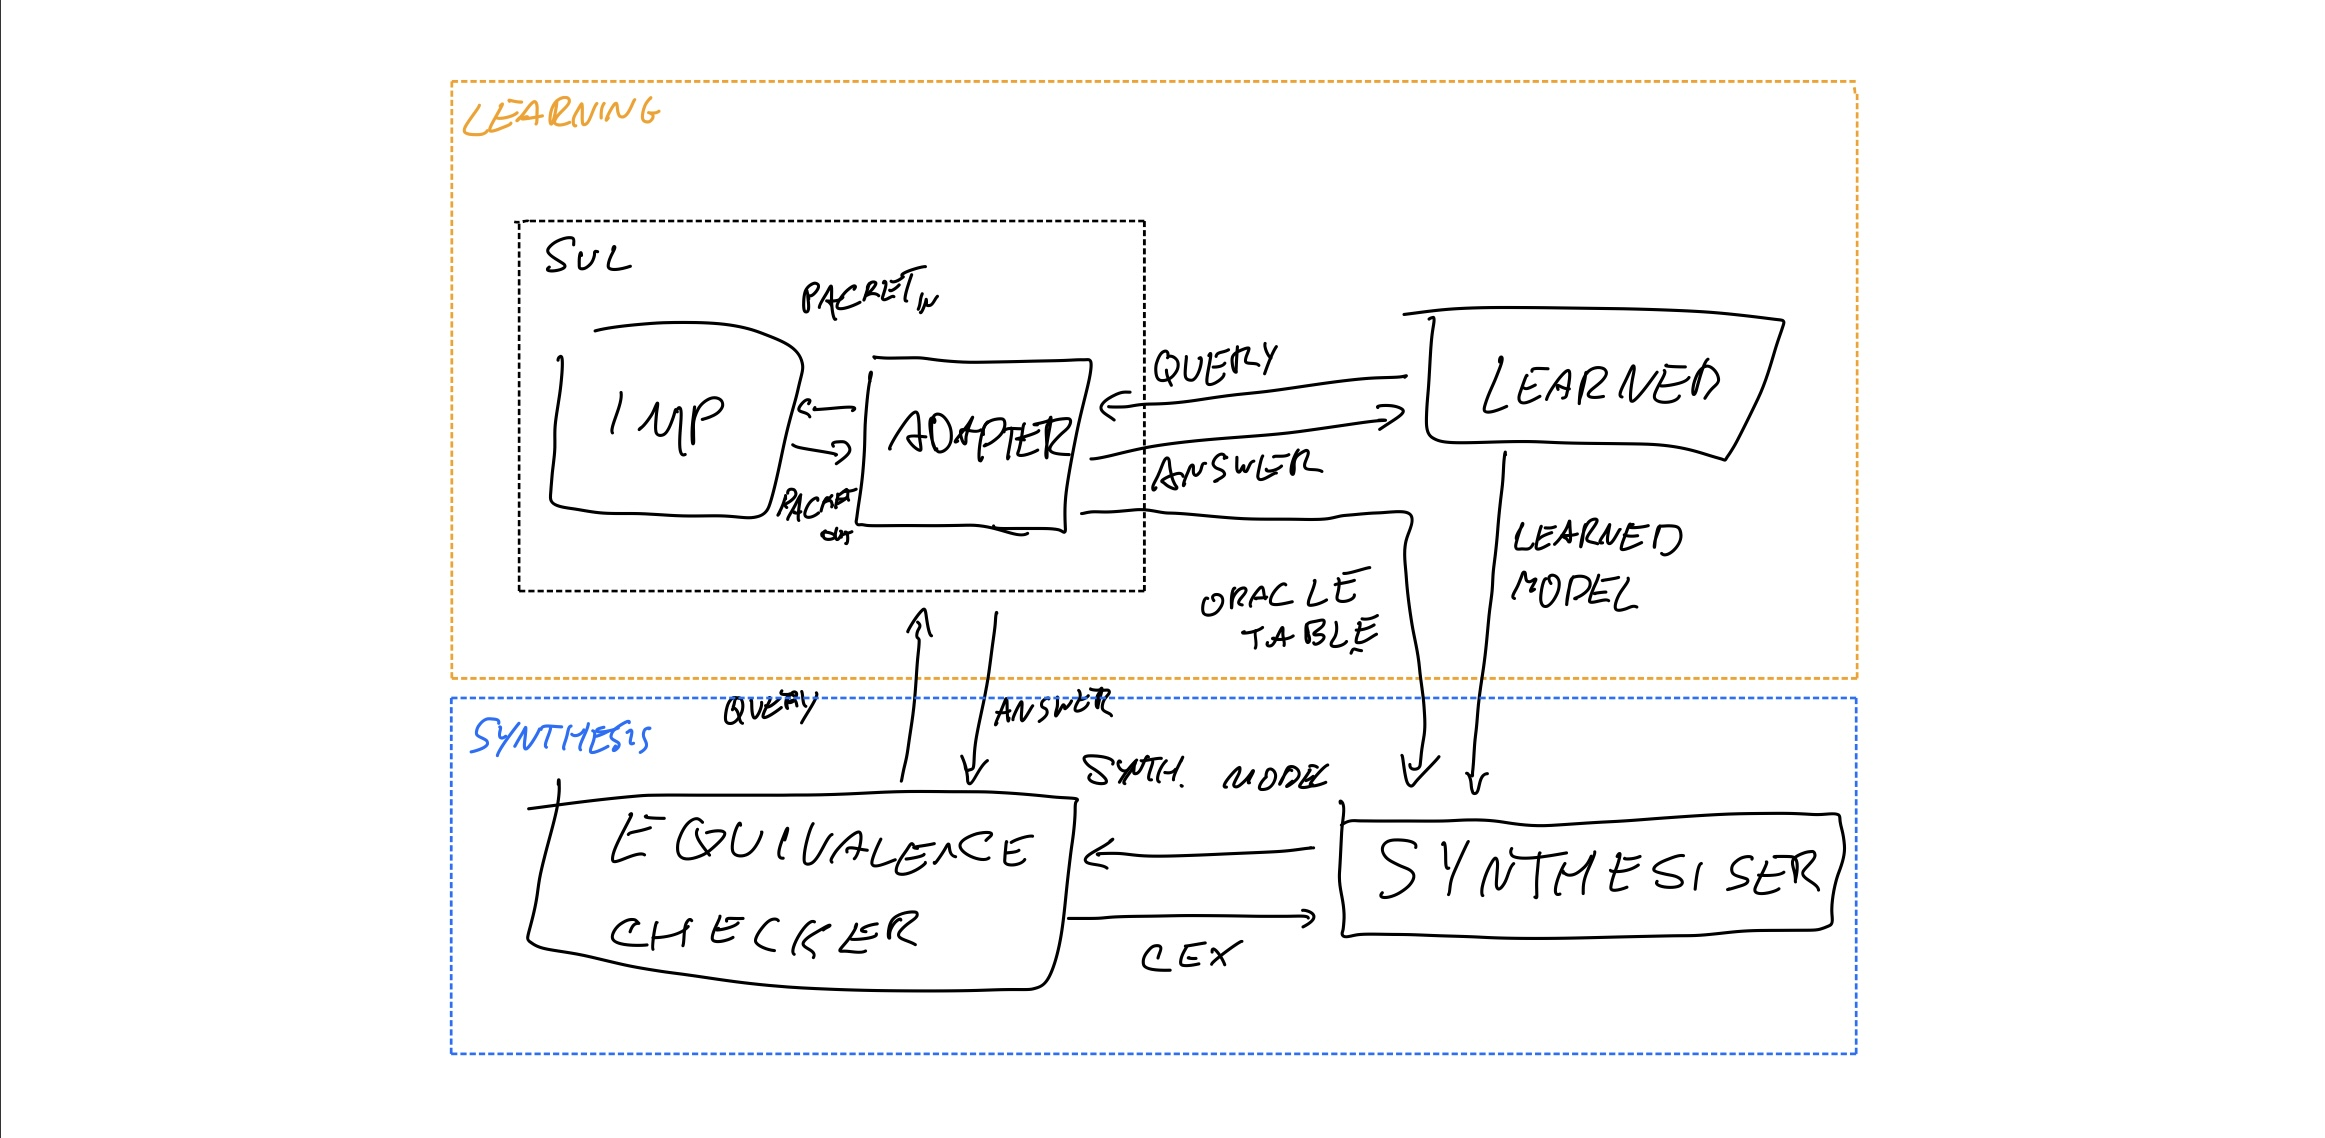
\includegraphics[width=\textwidth]{graphics/setup-drawing.jpg}


\tikzstyle{module} = [rectangle, draw,
    text width=5em, text centered, rounded corners, 
    minimum height=4em, node distance=5cm]

\tikzstyle{closemodule} = [rectangle, draw,
    text width=5em, text centered, rounded corners, 
    minimum height=4em, node distance=2cm]

\tikzstyle{line} = [draw, -latex']


\begin{figure}
    \centering
    \begin{tikzpicture}[node distance = 2cm, auto]
        % Place nodes
        \node [module] (sul) {System under learning};
        \node [module, right of=sul] (l*) {Learn Lib};
        \node [module, right of=l*] (synth) {Synthesizer};
        \node [closemodule, below of=l*] (tester) {Tester};
        
        \path [line] (sul) edge [bend left = 20] node {$a$-membership queries}(l*);
        \path [line] (sul) edge [bend right = 20] node {$a$-equivalence queries}(l*);
        \path [line] (l*) -- node {get $a$-machine}(synth);
        \path [line] (synth) edge [bend right = 20] node {get $w$-machine}(tester);
        \path [line] (tester) edge [bend right = 40] node {get c. example}(synth);
        \path [line] (sul) edge [bend right = 40] node {$w$-membership}(tester);
        
    \end{tikzpicture}
    \caption{
    It ugly.
    }
\end{figure}
Our algorithm starts by learning a mealy machine over the abstractions $\hat\Sigma$ of the input alphabet $\Sigma$ and $\hat\Gamma$ of the output alphabet $\Gamma$.
\subsubsection{Implementation}
The implementation is the original SUL we are attempting to learn. It can only communicate using the concrete alphabets $\Sigma$ and $\Gamma$, and so in our setup it interacts only with the adapter. This module can be conveniently swapped with any other implementation of the same protocol.
\subsubsection{Adapter}

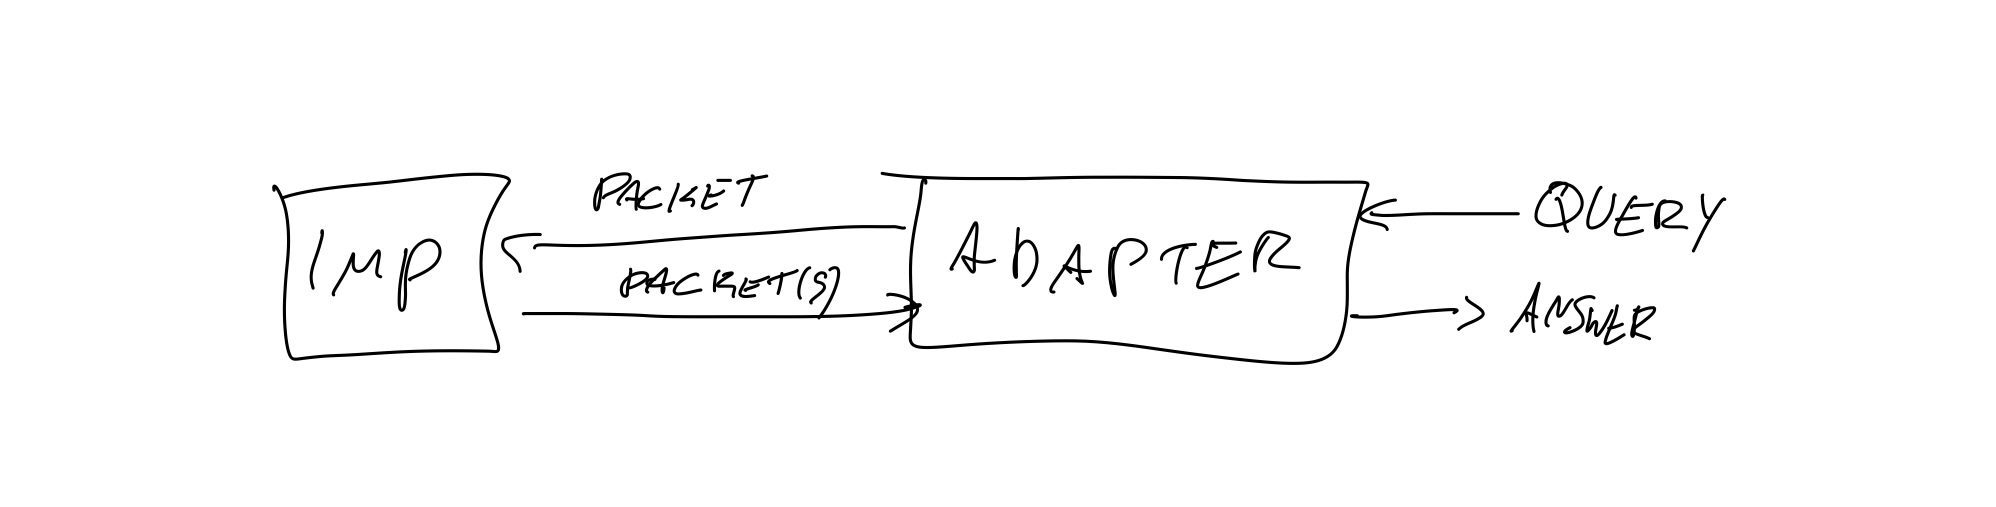
\includegraphics[width=\textwidth]{graphics/adapter-drawing.jpg}
A key part of interactive learning, is that the learner knows how to interact with the \sul. In some cases however, the \sul might use a very complex alphabet for communication, like specific packet formats and encrypted messages. 

We call the full detail represented in these symbols the concrete alphabets $\Sigma$ and $\Gamma$, for input and output symbols respectively. So even though a packet for example, is communicated as a sequence of binary digits $\mathbbm{2}^*$, the information those bits represent can be interpreted as a \textit{JSON} object containing the information of each field. 

In previous setups~\cite{tcp-learner} this component is called the \adapter, as it merely adapts the same data from a format to another, specifically, from sequences of concrete symbols to binary sequences. As such, it can be seen as a map of type $(\Sigma^* \times \Gamma^*) \to (\mathbbm{2}^* \times \mathbbm{2}^*)$.

We could then learn a state machine over these alphabets $\Sigma$ and $\Gamma$, knowing that they have a one-to-one native representation. However, often this is still not enough, as these concrete alphabets $\Sigma$ and $\Gamma$ might be too big for effective learning, or even infinite. As an example consider the concrete alphabets of a network packet format. These packets might have a \texttt{Packet Number} field, that is increasing and unique for each packet. We would then need to have an alphabet symbol for each of these packets, and even if that weren't an issue, this then combined with all the other possibilities for other counters gives us an extremely big alphabet. 

As such, it is common to learn instead over \textit{Abstract Alphabets} $\hat\Sigma$ and $\hat\Gamma$. These alphabets allow us to focus on the crucial aspects of the symbols by abstracting away details that would make the alphabet otherwise too big or infinite. This mapping however, is more complex than the \adapter, as the abstraction is a lossy conversion. When we abstract a concrete symbol to an abstract one, we are removing details we deem unnecessary for learning. However, these details are essential for the \adapter to communicate with the \sul, so we would need to determine this missing detailed information.

In the past~\cite{tcp-mapper}, this has been done with an extra element, the \mapper. The \mapper is an implementation of the Protocol logic that is able to abstract details away from a concrete alphabet to an abstract alphabet, and via the inverse construct these details, by running through the same logic that a normal implementation would. As an example, the \mapper in ~\cite{tcp-mapper} takes in a concrete TCP Packet TCP\{flags: \texttt{SYN}, Seq: \texttt{123}, Ack: \texttt{0}\} and produces an abstract TCP Packet TCP\{flags: \texttt{SYN}, Seq: $\top$, Ack: $\top$\} if it finds that the now abstract fields had valid concrete values. 

In the inverse, it has to be able to produce values that are valid, or invalid, as requested. As such, the \mapper can be seen as a function of type $(\hat\Sigma^* \times \hat\Gamma^*) \to (\Sigma^* \times \Gamma^*)$.

We found that this is a luxury that one cannot always afford. If the protocol relied on a logic of high complexity, including aspects like key derivation, encryption, or really symbols that contain a large number of fields to be abstracted, then this would mean programming an implementation logic of our own, that we trust to be correct and able to communicate with the \sul. 

There is a common expression in the field of Cryptography: \textit{Never roll your own Crypto.} This is because cryptographic algorithms tend to be of great complexity and have big consequences when they're incorrectly implemented. Thus it is preferred to use an existing implementation that has been widely used and so is more likely to be correct. We believe the same applies for the \mapper and \adapter in our case. 

As such, instead of having both a \mapper and then an \adapter, with a total of 2 maps being done of type $(\hat\Sigma^* \times \hat\Gamma^*) \to (\Sigma^* \times \Gamma^*) \to (\mathbbm{2}^* \times \mathbbm{2}^*)$, we instead have a single component, our \adapter, that is able to do a direct map of type $(\hat\Sigma^* \times \hat\Gamma^*) \to (\mathbbm{2}^* \times \mathbbm{2}^*)$, by combining the functionality of the two components used in ~\cite{tcp-learner}, while being able to keep a record of the intermediate values $(\Sigma^* \times \Gamma^*)$ used in the conversion. We call this the \at.

Furthermore, instead of coding all this logic ourselves, we adapted a common implementation that was specifically built for testing and is widely used by the implementers, and rely on it to both do the abstraction logic, and native formatting, as a normal implementation would. 

Now that we have constructed an abstraction that produces a finite alphabet, and we have effective ways of querying over this alphabet, we can learn this state machine using existing learning algorithms.

\subsubsection{Learner}
With our abstractions we are now learning a classic state machine, and so can use any of the classic algorithms available to us.

\subsubsection{Synthesizer}
Once we have learned a the abstract state machine we will enrich the edges with information to learn the more complex inputs and outputs. We do this by taking the learned machine and the examples gathered in oracle table by the abstract learner, 
and synthesizing a $w$-machine that correctly produces the input and output examples.

\subsubsection{Equivalence Checker}
Once we have synthesized a $w$-machine we then generate input examples from our machine, 
pass this input into the system under learning,
and determine if the combined input and output are accepted.

\subsection{Minimal Example}
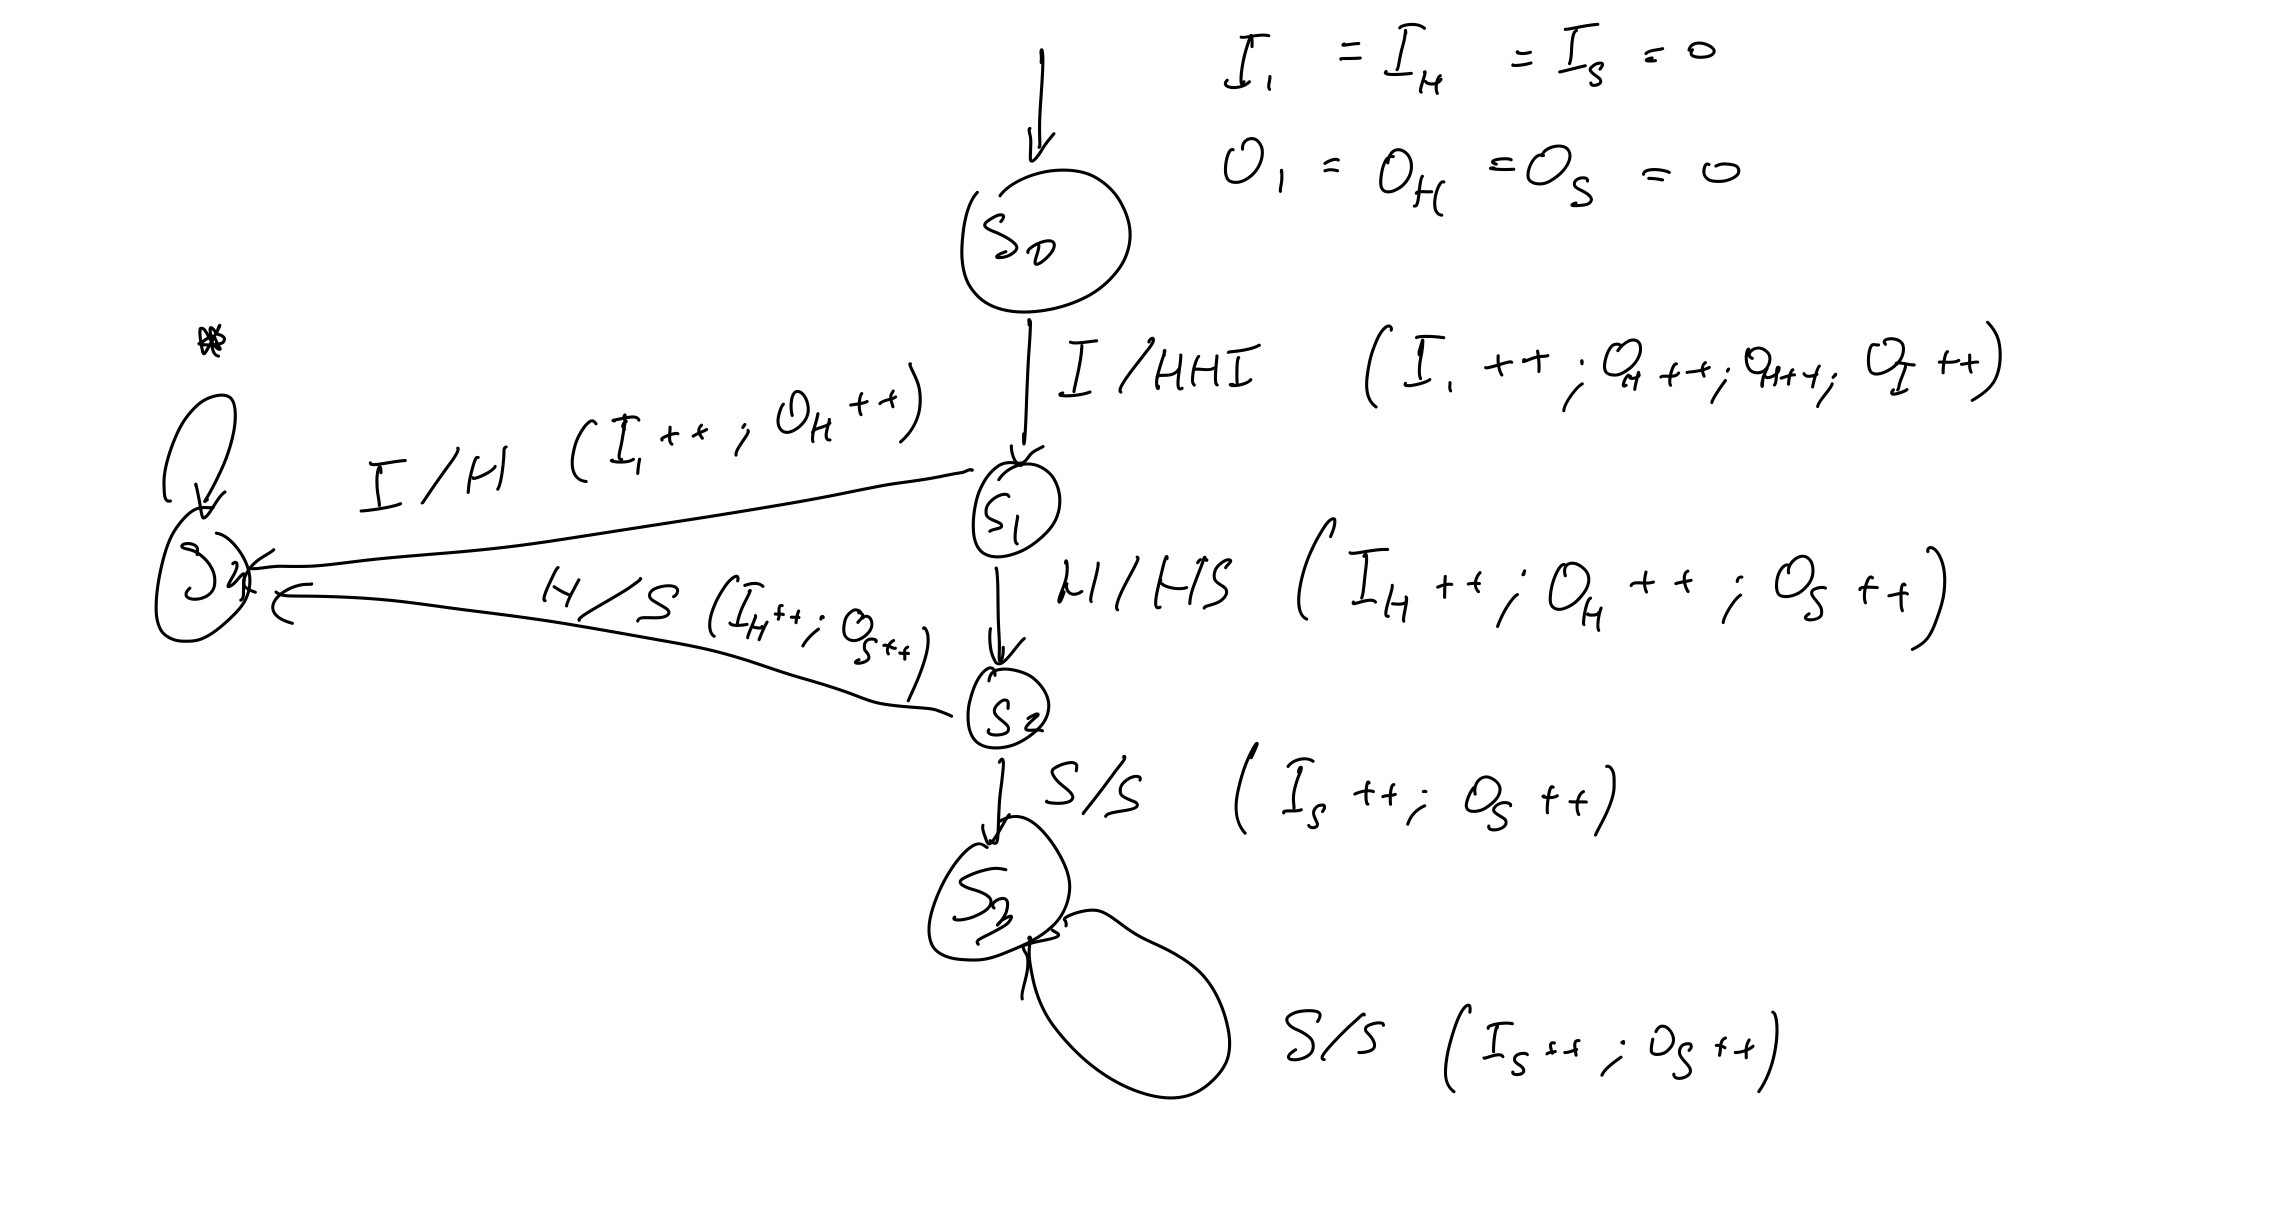
\includegraphics[width=\textwidth]{graphics/example-drawing.jpg}

%Informal problem def. - Explain the need for abstraction when learning, show how this removes information, demonstrate how this can sometimes be recovered with synthesis.  

%example + corresponding automaton. - simple example of the Big Counter Automaton, preferably abstract enough that it doesnt require background knowledge of the language.

%Eventually needs to have a run through of the algo – demonstrate automaton changing as the algorithm runs. 

\subsection{The Big Idea}

\section{Problem definition}


\subsection{$w$-machines}
\begin{definition}[Variable Set]
A variable set is a set of labels $V$. A variable set can be interpreted with an interpretation function, taking labels to integers: $\llbracket \cdot \rrbracket : V \to \mathbb{Z}$.
\end{definition}

\begin{definition}[Linear Relation Set]
A linear relation set is a $4-$tuple $(L, O, C, R)$,
where $L$, $C$, and $R$ are variable sets,
and where $O : (\B)^{\Z \times \Z}$ is a set of binary operators over the integers to the booleans.
It is defined as the following set of expressions:
$$\{l \oplus r + c : l \in L, \oplus \in O, c \in C, r \in R\}$$
\end{definition}

\begin{definition}[Transition]
A transition is considered over four variable sets:
\begin{itemize}
\item $I$, the input variable set, which are the set of fields in each input token
\item $O$, the output variable set, which are the set of fields in each output token
\item $R$, the register set, which is the set of registers
\item $C$, the constant set, a set of background constants
\end{itemize}
These variable labels are used in three linear relation sets:
\begin{itemize}
    \item $\phi = I \times \{\le, \ge\} \times R \times C$, which intuitively is the set describing the guard of the transition.
    \item $\chi = R'\times \{=\}\times R\times C$, which intuitively is the set describing the update to the registers, with $R'$ being the same set as $R$, but updated versions.
    \item $\chi = R'\times \{=\}\times O\times C$, which intuitively is the set describing the output values. 
\end{itemize}
The three sets are used in transition denoted as follows:
$$ p \xrightarrow{\phi / \chi / \psi} q$$
Such that if in state $p$ and $\phi$ is true, we go to state $q$ and require $\chi \wedge \psi$.
\end{definition}

\begin{definition}[$w$-machine]
A $w$-machine is given by a tuple:
$(I, O, R, r_0, Q, q_0, \Delta, F)$
where $I$ is the set of input variable labels,
$O$ is the set of output variable labels,
$R$ is the set of register variable labels,
$r_0 : R \to \mathbb{Z}$ takes registers to their initial values,
$Q$ is the set of states,
$q_0$ is the initial state,
$F \subseteq Q$ is the set of final states,
and transitions as defined in the previous given by $\Delta \subseteq Q \times \phi \times \chi \times \psi \times Q$.
Provided the actions defined for transitions (including the update of registers),
the execution of the machine is what you would expect from a transducer.
\end{definition}

\begin{definition}[Problem Definition]
Assume we have a system under learning, which can be described with a $w$-machine $W$. Furthermore assume we have an oracle for the system under learning $O : I^* \to \{\top, \bot\}$, such that the oracle decides membership in $W$ (i.e. $\lambda w. w \in \mathcal{L}(W) = O$). We wish to recreate the $w$-machine with the oracle.
\end{definition}

\section{Learning w-machines}

In this section, we present the algorithm for learning w-machines from the oracle.
First we show how the alphabets involved in the learning problem can be abstracted to learn a finite state machine
without counters in Section~\ref{}. Second, we present an algorithm that given an abstract finite state machine
and the corresponding set of concrete examples generalizes the finite state machine to a w-machine that is consistent
with the concrete examples and it uses counters in Section~\ref{}.

\subsection{Learning abstract w-machines}


\begin{definition}
An abstraction function $\alpha : (\Sigma \times \Gamma) \to (\hat\Sigma \times \hat\Gamma)$ maps alphabets $\Sigma$ and $\Gamma$ to finite alphabets $\hat\Sigma$ and $\hat\Gamma$, respectively.
\end{definition}
Note: maybe gamma doesn't need to be finite. Investigate

\begin{example}
TODO show example of alpha using example in sec 2
\end{example}

\begin{definition}[Abstract w-machine]
An Abstract $w$-machine $M_\alpha$ is a 6-tuple $(S, S_0, \hat\Sigma, \hat\Lambda, T, G)$, such that:
\begin{itemize}
    \item $S$ is a finite set of states. 
    \item $S_0$ is the initial state such that $S_0 \in S$.
    \item $\hat\Sigma$ is the abstract input alphabet. 
    \item $\hat\Gamma$ is the abstract output alphabet.
    \item $T$ is the transition function $T \colon S \times \hat\Sigma \to S$.
    \item $G$ is the output function $G \colon S \times \hat\Sigma \to \hat\Gamma$.
\end{itemize}
\end{definition}

\begin{definition}[Abstracting a w-machine]
Given an abstraction function $\alpha$ from $(\Sigma,\Gamma)$ to $(\hat\Sigma,\hat\Gamma)$,
and a w-machine $M=(I, O, R, r_0, Q, q_0, \Delta, F)$
the abstract w-machine $M_\alpha=(S, S_0, \hat\Sigma, \hat\Gamma, T, G)$.
\end{definition}

Something about $M_\alpha$ simulating $M$.

Using this, we can now try to learn $M_\alpha$, but to do so we need an oracle for it.

Explain how to get abstract membership queries from the oracle you have.
\begin{theorem}
We will  learn the abstract w-machine for the given machine using the oracle
\end{theorem}


Note that an abstract w-machine is equivalent to a classic mealy machine, which we can learn using existing algorithms.

\subsection{Learner interface}
Our learning process starts with the classic \emph{Minimally Adequate Teacher} (MAT) framework. We have a learner that is attempting to infer a model Abstract $w$-machine via two kinds of queries:
\begin{itemize}
    \item \textbf{Membership Queries} of the type $w_O = mq(w_I)$ where $w_I \in \hat\Sigma^+$ and $w_O \in \hat\Gamma^+$. In practise, these are single $w_I / w_O$ traces of the system that allow the learner to acquire knowledge about the behaviour of the SUL so that it can build an hypothesis model $H$.
    \item \textbf{Equivalence Queries} of the type $w_I / w_O = eq(H)$ where $H$ is an hypothesis model the learner believes to be correct and wants to know if it is indeed equivalent to the SUL, the answer $c$ is a counterexample trace that is present in the SUL, but not in the hypothesis model $H$, thus proving the hypothesis is not correct. If no counterexample is returned, theoretically the model is equivalent to the system, and thus correct. In practice, Equivalence Queries would require an Equivalence Oracle omniscient of the SUL, and if we had that, we wouldn't have to learn the system in the first place. However, we can use heuristic Equivalence Oracles such that when a counterexample is returned, it is indeed guaranteed to be a valid counterexample, but the absence of a counterexample no longer guarantees equivalence. This can still give us PAC guarantees.
\end{itemize}

With oracles capable of answering the two types of queries mentioned above, we are able to make use of a black-box learning algorithm to learn a model of the SUL. There are many different algorithms that can learn a model with access to these oracles using different backing data structures and with different efficiencies, however they almost always follow a similar loop based structure as such:

\textbf{TODO}: Make sure this makes sense for at least both L* and TTT.

\begin{algorithm}[H]
\KwResult{Learned Model}
L := Learner($\hat\Sigma$)\;
\While{True}{
    $W_I$ := L.buildQueries()\;
    \If{$W_I$ = $\O$ }{
        H := L.hypothesis()\;
        \If{$w_I / w_O$ := eq(H)}{
            L.consider($w_I / w_O$)\;
            continue\;
        }
        \Return{H}\;
    }
    \For{$w_I \in W$}{
        $w_O$ := mq($w_I$)\;
        L.consider($w_I / w_O$)\;
    }
}
\caption{Black-box learning loop}
\end{algorithm}

\subsection{Generalizing abstract w-machines to w-machines}
We have now successfully learned an Abstract $w$-machine through the abstraction alphabets $\hat\Sigma$ and $\hat\Gamma$, however we still want to enrich this model by generalising it to a $w$-machine.

\begin{definition}[$w$-machine SMT problem]
$w$-machine SMT problem is given by the function 
$$\mathcal{S} : (A \times E \times [0, K) \times [0, R) \times C) \to \{\bot\} \sqcup (2^{Q \times Q \times [0, K) \times O \times \{\phi, \chi, \psi\}}, [0, R) \to \mathbb{Z})$$
Where:
\begin{itemize}
    \item $A$ is the finite automata learned in the previous
    \item $E$ is the set of examples and counter-examples given
    \item $K$ is the number of edges between any two states
    \item $R$ is the number of registers to assume for synthesis
    \item $C$ is the set of constants
    \item $Q$ is the set of states of $A$
    \item $O$ is the set of operators given in $H(P,Q)$ in the guard definition
    \item $\phi$, $\chi$, and $\psi$ are just labels.
\end{itemize}
It asks to find a subset $I$ of $Q \times Q \times K \times O \times \{\phi, \chi, \psi\}$,
and initial register assignment $D: [0, R) \to \mathbb{Z}$,
such that an edge between two nodes in $A$ with label $f$
is necessary and sufficient between two nodes in the synthesized machine with requirement that label $f$ also be matched by the input. 
If it can't, it returns $\bot$: failure.
This can be written as a very large SMT problem.
\textbf{TODO: probably not, but maybe put problem in?}
\end{definition}

The idea is we enrich the learned automata with extra information along the edges that can use registers to match extra information of the language (information that can not be represented with a finite state machine).

\subsection{How to generalize abstract w-machines to w-machines}
\begin{algorithm}[H]
\caption{synthesis algorithm}
\For{$e, r, c \in \N^3$, diagonally}{
    $v \gets S(A, examples, e, r, c)$\;
    \If{$v = \bot$}{
        \textbf{continue}\;
    } \Else{
        $m \gets$ machine gathered from $v$\;
        \For{$(i, o) \in \lang{m} \cup \lang{\neg m}$}{
            \If{$(i, o) \in \lang{m} \wedge (i, o) \not\in \lang{s}$}{ \tcp*{$s$ is the system under learning}
                add $\neg(i, o)$ to $examples$ \tcp*{that is, as a counter example}
                \textbf{break}\;
            } 
            \If{$(i, o) \not\in \lang{m} \wedge (i, o) \in \lang{s}$}{
                add $(i, o)$ to $examples$\;
                \textbf{break}\;
            }
        }
    }
}
\end{algorithm}

Soundness theorem: the synthesize machine will always be correct upto all examples seen

% This is pretty straight forward: we require in SMT problem all examples are right and that the abstract automata is right

Completeness theorem: If your automata can be represented by abstracted 
to a learnable automata, then your automata can be synthesized using a learned automata to define its structure. 

\subsubsection{Proof of completeness}

\begin{lemma}[The right NFA from a DFA]
We can synthesize $M$, an $NFA$,
over a finite alphabet $\alpha$ upto state-isomorphism using $1$ register and $|M|$ edges.
\end{lemma}

Suppose we are synthesizing a big-counter machine $A$ also over $\alpha$ starting with a graph structure given by a DFA representation of $M$, called $B$, that has an isomorphism between states of $M$ and states and registers of $A$.
Let the states of the machines be given by $Q_M$ and $Q_A$ respectively, and the same with $\Delta_M$ and $\Delta_A$.
Assume any mapping from $Z : Q_M \to \mathbb{Z}$.
Assume, further a mapping from $D : Q_m \to 2^{Q_a}$, which takes a $q \in Q_m$ to a subset states $q_a$ of $Q_a$ such that there exists a string $s$ where $M[s] = q$, and $q_a = B[s]$.
Then, we can map each state $m$ in $M$ to a register value $R(m)$,
and each edge $(q_m, c, p_m)$to a set of $w$-machine edges: $\{(q_a, c \wedge r = Zq, p_a) : p_a \in Dp_m, q_a \in Dq_m\}$.
Thus if we are in state $q_a$ and register value $r$, with input $c$, we will go state $p_a$ and register value $r'$ if there is an edge $(Dr, c, Dr')$ in $M$, and same visa versa. $\square$ 

Assuming we can do the above, then we can learn all additional data across the edges with $r+1$ registers and $|S|$ states, where $r$ is the number of registers used by the machine $S$.

Furthermore, there are finite machines for every given number of registers and states (essentially powerset over relations including bit-vector values, product of this over three predicates, is big but finite). As we will eventually always get each trace, we will eventually get a set of traces that shatters the set of machines down to just one machine. 

\subsubsection{Proof of Soundness}

Positive examples are only added if they are actually generated by the system under learning.
Negative examples are only tentatively added, so that if they are seen later, those negative example are added.
Thus, we only synthesize machines that behave correctly according to all examples we've seen,
and if we assume a negative example, and we  ever learn that is accepted, then we remove it. 

% It got a little late to type this out, but this requires two parts, first we show that we learn a DFA abstract mealy machine, and two that through registers and edges we can simulate what ever the orginal DFA was. So, eventually we'll synthesize the right machine

\section{Experiments}
Examples of research questions regarding the usefulness and power of this learning method. 
\begin{itemize}
    \item RQ1: Can we learn a $w$-machine that cannot be learned as a regular machine?
    \item RQ2: Can we extract useful specification properties from this machine?
    \item RQ3: Can we learn a $w$-machine using only the queries used in learning the abstract $w$-machine?
\end{itemize}

To evaluate these questions, we use our learning technique to model check implementations of the QUIC Protocol. QUIC is a new general-purpose transport layer network protocol that aims to improve connections by decreasing the amount of handshakes required for different protocol layers, eliminating head-of-line blocking, and allowing for connection recovery even when the client changes networks. QUIC enables all this while providing packet encryption at the transport layer. 

One can picture QUIC as a \emph{super protocol}, as it eliminates the needs for so many other network layers by incorporating TLS1.3 in the packet encryption, and providing NAT rebinding resilience. As such, the QUIC Protocol carries an unusually high degree of complexity while having the goal of, with time, being the \emph{de-facto} standard for HTTP connections. This makes it an ideal candidate for verification. 

In this paper we will be verifying two main implementations of the IETF QUIC Protocol (Draft 29):
\begin{itemize}
    \item \textbf{Quiche}: Cloudflare's QUIC Implementation that allows QUIC connections to any website protected by Cloudflare network. QUIC support has been enabled automatically for Cloudflare-backed websites, with website administrators having the option of manually disabling it. Cloudflare's CDN supports over 25 million websites, so we believe it is crucial for this implementation to be as correct as possible.
    \item \textbf{Google QUIC}: Google's QUIC Implementation that runs on Google servers and on Chromium browsers. Since October 7 of 2020, 25\% of Google Chrome users had QUIC support enabled by default, with that proportion increasing over the followed weeks. As Google Chrome is the most widely used web browser in the world, we consider the correctness of this implementation to be crucial too.
\end{itemize}

To evaluate the correctness of these implementations we selected a subset of properties from the specification to be verified:

\begin{enumerate}
    \item An endpoint MUST open streams of the same type in increasing order of stream ID.
    \item Before a stream is created, all streams of the same type with lower- numbered stream IDs MUST be created.
    \item A sender MUST ignore any MAX\_STREAM\_DATA or MAX\_DATA frames that do not increase flow control limits.
    \item An endpoint MUST NOT send data on a stream at or beyond the final size.
    \item A receiver MUST ignore any MAX\_STREAMS frame that does not increase the stream limit.
    \item The sequence number on each newly-issued connection ID MUST increase by 1.
    \item A server MUST set the Destination Connection ID it uses for sending packets based on the first received Initial packet.
    \item A QUIC endpoint MUST NOT reuse a packet number within the same packet number space in one connection.
    \item ACK Frames and Packet Protection ACK frames MUST only be carried in a packet that has the same packet number space as the packet being ACKed.
    \item A server MUST treat receipt of a HANDSHAKE\_DONE frame as a connection error of type PROTOCOL\_VIOLATION.
\end{enumerate}


\pagebreak
\section{OLD Problem definition (deprecated below here:}

TODO: preface this all section with an intuition of what we are about to read in English

\subsection{Automata}
We define a linear automata as 
a tuple $(Q, \Delta, q_0, v_0, F, i, o, c)$.
Where $Q$ is a set of states.
$q_0$ is the initial state.
$v_0$ is the initial register values.
$F$ is a field.
$i$ is the size of input vectors,
$o$: output vectors,
$c$: constraints.
$\Delta$ is a set of tuples denoting transitions $(s, G_{c, i+r}, G_c, O_{o, i+r}, O_o, U_{r, r}, U_r, s')$.

If in state $s$, 
and register vector $v$,
with input $i$,
we can traverse a transition $(s, G_m , G_v, O_m, O_v, U_m, U_v, s')$ if $G_m(v \lozenge i) \leq G_v$ (here, $\lozenge$ denotes vertical concatenation).
This outputs $O_m(v) + O_v$ as the output vector, updates the registers to $U_mv + U_v$, and takes us to state $s'$.
This process continues to end of input
or till no edge accepts out of current state.
\subsection{Big Counter Automata}
Big counter automata are a refinement on the previous that tightly contain the languages we're considering.
They are regular multi-counter automata, 
but with the ability to take non-deteriministic positive and negative steps:
this simulates many things we see in the processes that we are learning.
Examples of this are a time counter increasing or non-sequential, but increasing, packet numbers.

\begin{definition}
Big step automata is a $X-$machine
with data $X = \mathbb{N}^* \times I \times O$ 
-- a finite number of counters with an input and output.
The input and output are both a finite list of numbers,
but possible different sizes.
We discuss the $i$-th counter with $X_i$.
We discuss the $j$-th input value for state $x$ with $X_I_j$,
and similarly with output: $X_O_j$
A transition in a BSA from any two states $c$ to $d$
must be a relation $(x, x')$ on $X$ definable with a conjunction of
some of the following formulae for any $i$ and $j$:
$x'_i = x_i + \{-1, 0, 1\}$ or 
$x'_i >/< x_i$ or 
$x'_O_j = x_i$ or
$x'_O_j = c$ (a constant) or
$x_I_j =/</> x_i$.
Also, the domain of the relation must be defineable with
some convex interval of the counters.
And, the domains of the relations from some node must be disjoint.
\end{definition}


\subsection{Approximation}
Counter is a language that accepts a series of ones, 
increasing a register for each one,
and outputting zero.
When a zero is passed, 
the register value is output, and then reset.
This is a simple example of the kind of automata the we seek to learn.

In theory, though impossible,
we want to learn an entire Mealy machine for this language.
This machine still has traditional DFA edges,
but has one state for each value of the counter and an infinite output alphabet.

We can learn, however, some neighborhood of the the states about the initial state.
If we learn a big enough neighborhood, we'll see that a lat of the graph is compressible.
A graph is compressible if many of its nodes have similar neighborhoods.
For example,
the counter language will have many neighborhoods of the shape:
a transition from some node by 1,
a transition to some node by 1,
and transition to the initial node by some number.
What we want to do is take an mealy machine learned by the learner
that approximates the conceptual infinite mealy machine by some finite number of states,
and induce a mealy machine with counters that is equivalent to the infinite mealy machine.

\begin{definition}{Synthesis problem}
Suppose the learner has learnt a mealy machine \mathcal{M}.
And this machine is an approximation for the SUL \mathcal{S}.
We seek to create a big step automata \mathcal{B}
which is equivalent to \mathcal{M},
using induced patterns from \mathcal{S}.
\end{definition}



%

\tikzstyle{module} = [rectangle, draw,
    text width=5em, text centered, rounded corners, 
    minimum height=4em, node distance=5cm]
\tikzstyle{close_module} = [rectangle, draw,
    text width=5em, text centered, rounded corners, 
    minimum height=4em, node distance=2cm]

\tikzstyle{line} = [draw, -latex']


\begin{figure}
    \centering
    \begin{tikzpicture}[node distance = 2cm, auto]
        % Place nodes
        \node [module] (sul) {System under learning};
        \node [module, right of=sul] (l*) {Learn Lib};
        \node [module, right of=l*] (synth) {Synthesizer};
        \node [close_module, below of=l*] (driver) {Driver};
        \node [close_module, below of=synth] (problemer) {Problem Finder};
        
        \path [line] (l*) edge [bend left = 20] node {m and e queries}(sul);
        \path [line] (sul) edge [bend left = 20] node {counter-examples}(l*);
        \path [line] (l*) -- node {NFA}(synth);
        \path [line] (driver) edge [bend right = 0] node {Exploit goal}(problemer);
        \path [line] (synth) edge node {Synthesized model}(problemer);
        \path [line] (synth) edge [bend right = 60] node {Membership queries}(sul);
    \end{tikzpicture}
    \caption{
    Between the system under learning and learn lib is the familiar MAT learning model.
    Once learned, an non-deterministic finite automata model of the SUL is passed to the synthesier.
    The CEGIS synthesizer then tries to synthesize a refinement of the NFA to a mealy machine with registers, using random walks of synthesized mealy machines to see if they are accepted by system under learning.
    Combined with an an exploit goal from the driver (e.g. explode memory), the problem finder tries to find a trace that achieves the exploit or show proof otherwise.
    }
\end{figure}
%
\begin{algorithm}[H]
% \SetAlgoLined
\SetKwInOut{Input}{Input}
\SetKwInOut{Output}{Output}
\Input{A system under learning $\mathcal{S}$ and an exploit goal $\mathcal{E}$}
\Output{Returns a failure, a exploitive trace, or a proof of non-exploit on the learned model}
get learned NFA, $\mathcal{N}$, with LearnLib($\mathcal{S}$)\;
get synthesized model or error $\mathcal{M}$ with CEGIS($\mathcal{N}$, $\mathcal{S}$), and halt if error\;
return either exploitive trace or proof of non-exploit of synthesized model with ProblemFinder($\mathcal{M}$, $\mathcal{E}$). 
\end{algorithm}
\subsection{Learning}
\input{Learning}

\end{document}
